\documentclass[10pt,letterpaper]{article}

  %%%%%%%%%%%%%%%%%%%%%%%%%%%%%%%%%%%%%%%%%%%%%%%%%%%%%%%%%%%%%%%%%%%%%%%%%
  % \setallmargins{1in}

  \usepackage[margin=1in]{geometry}

  \usepackage{fancyhdr,lastpage}
  \pagestyle{fancy}

  \fancyhead{}
  \fancyfoot{}

  \renewcommand{\headrulewidth}{0.5pt}
  \renewcommand{\footrulewidth}{0pt}

  \rhead{Kesari}
  \lhead{NSF Proposal, Fall 2017}
  \cfoot{\thepage}
  %

  %%%%%%%%%%%%%%%%%%%%%%%%%%%%%%%%%%%%
  \newcommand{\required}[1]{\section*{\hfil #1\hfil}}
  \renewcommand{\refname}{\hfil References Cited\hfil}
  \bibliographystyle{unsrt}

  \renewcommand{\familydefault}{\sfdefault}
  \usepackage[T1]{fontenc}
  \usepackage[scaled=1]{helvet}

  \usepackage[svgnames, table]{xcolor}
  \usepackage{array}
  \usepackage{environ}
  \usepackage{tikz}
  \usepackage{verbatim}
  \usepackage{float}
  \usepackage{amsmath, amssymb}
  \usepackage{mathtools}
  %\usepackage[usenames]{color}
  \usepackage{graphics,graphicx,wrapfig}
  \usepackage[bf,small,compact]{titlesec} % Allows customization of titles
  \usepackage[colorlinks=false]{hyperref}
  %\usepackage[notref,notcite]{showkeys}
  %\usepackage{showlabels}
  %\usepackage{labels}
  %\hypersetup{colorlinks=false}
  \usepackage{todonotes}
  \usepackage[font=small]{caption}
  \usepackage[sort&compress]{natbib}
  \urlstyle{same}
  \usepackage[hang]{footmisc}
  \usepackage{enumerate}
  \usepackage{epigraph}
  \usepackage{enumitem}
  \usepackage{tcolorbox}
  \usepackage{mdframed}

  \definecolor{orange}{cmyk}{0,0.5,1,0}
  \definecolor{HKblue}{cmyk}{65,4,0,0}
  \definecolor{HKblue2}{cmyk}{100,0,0,0}

  \usetikzlibrary{shapes,snakes}

  % User defined commands
  \newcommand{\unit}[1]{\ensuremath{\, \mathrm{#1}}}
  \newcommand{\bs}[1]{\ensuremath{\boldsymbol{#1}}}
  \newcommand{\mc}[1]{\ensuremath{\mathcal{#1}}}
  \newcommand{\norm}[1]{\ensuremath \lVer #1 \rVert}
  \newcommand{\rhat}{\hat{\rho}}
  \newcommand{\figwidth}{2.2in}

  \renewcommand{\comment}[2]{{\color{#1} $\blacksquare$ \footnote{\noindent \color{#1}#2} }}
  \newcommand{\commenti}[2]{{\color{#1} $\blacksquare$  \color{#1}#2} }
  \newcommand{\commentm}[2]{{\color{#1} $\blacksquare$  \marginpar{\color{#1}#2} }}

  \newcommand{\tikzarrow}{
  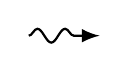
\begin{tikzpicture}
   \draw [decorate, decoration={snake}, black,  thick ] (0.1,0)--(0.8,0)  ;
   \draw [ black,  very thick,  -> , baseline, -latex] (0.8,0)--(1.0,0) ;
  \end{tikzpicture}
  }

  \usepackage[normalem]{ulem}

  \setlength{\parindent}{0cm}
  \setlength{\parskip}{0.4em}

  \titleformat{\section}
    {\normalfont\fontsize{12}{12}\bfseries}{\thesection}{1em}{}



  \usepackage{tabu}
  \usepackage{longtable}
  \usepackage[table]{xcolor}

  \definecolor{tableHeader}{RGB}{211, 47, 47}
  \definecolor{tableLineOne}{RGB}{245, 245, 245}
  \definecolor{tableLineTwo}{RGB}{224, 224, 224}

  \newcommand{\tableHeaderStyle}{
      \rowfont{\leavevmode\color{white}\bfseries}
      \rowcolor{tableHeader}
  }

  \usepackage{multirow}
  \begin{document}
%%%%%%%%%%%%%%%%%%%%%%%%%%%%%%%%%%%%%%%%
\setcounter{page}{1}

\begin{center}
  \fontsize{12}{2em}
  \selectfont
  Understanding the origin of toughness enhancement in complex architectured ceramic composites by developing and using an anisotropic variational fracture theory
\end{center}
%%%%%%%%%%%%%%%%%%%%%%%%%%%%%%%%%%%%%%%%

%%%%%%%%%%%%%%%%%%%%%%%%%%%%%%%%%%%%%%%%%%%%%%%%%%%%%%%%%%%%%%
%%%%%%%%%%%%%%%%%%%%%%%%%%%%%%%%%%%%%%%%%%%%%%%%%%%%%%%%%%%%%%
%%%%%%%%%%%%%%%%%%%%%%%%%%%%%%%%%%%%%%%%%%%%%%%%%%%%%%%%%%%%%%
\section{Introduction}
  %%%%%%%%%%%%%%%%%%%%%%%%%%%%%%%%%%%%%%%%%%%%%%%%%%%%%%%%%%%%%%
  \subsection{Research objective}
    \label{s:ro}
    \emph{We seek to derive fundamental scientific knowledge of how architectural motifs in 3D, ceramic composites affect their toughness and damage tolerance.}

    In most engineering materials strength and toughness are mutually exclusive~\cite{ritchie2011conflicts}. This issue is a critical bottleneck for aerospace, transportation, and energy production technologies. Structural biological materials (SBs), such as bone and shell, are an interesting class of materials that could provide strategies for overcoming this issue. While SBs are often composed of >95\% brittle ceramic material by volume, they have been shown to possess extraordinary toughness and damage tolerance while maintaining both strength and stiffness~\cite{barthelat2011toughness,rabiei2012nacre,currey2003well,wang2001deformation}. For example, the total energy dissipated during the fracture of nacre has been shown to exceed that of its constituent ceramic material, aragonite, by three orders of magnitude~\cite{currey1976further,Currey:1977wf}.  This effect is especially intriguing since it cannot be explained using basic composite mechanics ideas, such as the rule of mixtures (see Figure~\ref{f:hyp} (c))~\cite{wegst2015bioinspired}. This remarkable toughness and damage tolerance is believed to be a consequence of the SBs' complex, small-scale architectures (Figure~\ref{f:intro} (a)--(b)).
%
    \begin{figure}[h!]
      \centering
        \includegraphics[width=\textwidth, trim={0 0.0cm 0.0cm 0}, clip]{Figures/Introduction/IntroFig_V7.pdf}
        \caption{ \footnotesize The complex architecture of SBs and ceramic composites. (a) Cylindrical, concentric layers of silica in the spicules of the marine sponge \textit{Euplectella aspergillum} (modified from \cite{monn2015new}). (b) Brick-and-mortar architecture of calcium carbonate tablets in nacre (molluscan shell) (reprinted from \cite{ritchie2011conflicts}). (c) A SiC/graphite composite made using fibrous monolith construction techniques (reprinted from \cite{baskaran1993fibrous}).
          }
        \label{f:intro}
      \end{figure}
%
    Structural biological materials are composites that consist of a ceramic and an organic phase mixed in intricate 3D patterns~\cite{mayer2005rigid,meyers2013structural}. The arrangement of these phases is referred to as the SB's architecture.  Currently, there are no mechanics of materials theories that can connect how different architectural motifs affect large-scale toughness in SBs, or complex composites in general. That is, there are no analytical or numerical solutions that can help us  answer questions such as (Q.1) Which architectural motifs are best for enhancing toughness for a given system of constituent materials, interface properties, and mechanical loads? (Q.2) Are the mechanical properties of the interfaces actually more important than the architectural motifs for enhancing toughness? (Q.3) What are the upper bounds to the toughness enhancements that architectural motifs can provide?

    The key hurdle that has prevented the translation of the remarkable toughness enhancement seen in SBs to engineering materials is the lack of fundamental scientific knowledge connecting small-scale architectural motifs to large-scale toughness. This project's research objective is motivated by the need to fill this knowledge gap.

  %%%%%%%%%%%%%%%%%%%%%%%%%%%%%%%%%%%%%%%%%%%%%%%%%%%%%%%%%%%%%%
  \subsection{Research strategy}
    \label{s:strat}
    \emph{We will develop a new mechanics of materials theory---anisotropic regularized variational fracture theory (aRVFT)---that will enable accurate numerical simulations of the evolution of complex crack networks in SBs and SB-inspired composites. We will then demonstrate the predictive capability of aRFVT by using it as a tool to understand the connection between architecture and toughness in a model SB.}%ø

    The primary challenges of this research strategy are: 1) developing a theory and computational framework that accurately predicts crack evolution, without being prohibitively computationally expensive (see \S \ref{s:A1}), and 2) fully characterizing the architecture and material properties of a SB so that it's fracture behavior can be modeled using the aRVFT (see \S \ref{s:A2}).

  %%%%%%%%%%%%%%%%%%%%%%%%%%%%%%%%%%%%%%%%%%%%%%%%%%%%%%%%%%%%%%
  \subsection{Research hypothesis}
    \label{s:hyp}
    \emph{We hypothesize that the toughness enhancements observed in SBs and SB-inspired composites are consequences of the interfaces within them acting like traps and mazes. While the stiff phases fail through brittle fracture, the interfaces trap the cracks and make them consume much more energy to spread across the specimen. They do this primarily by pinning, deflecting, and splitting the cracks (see Figures~\ref{f:hyp}(a)--(b) and ~\ref{f:sim}(a))~\cite{gao1989first,dalmas2009crack,gu1997crack}.}
%
    \begin{figure}[h!]
         \centering
           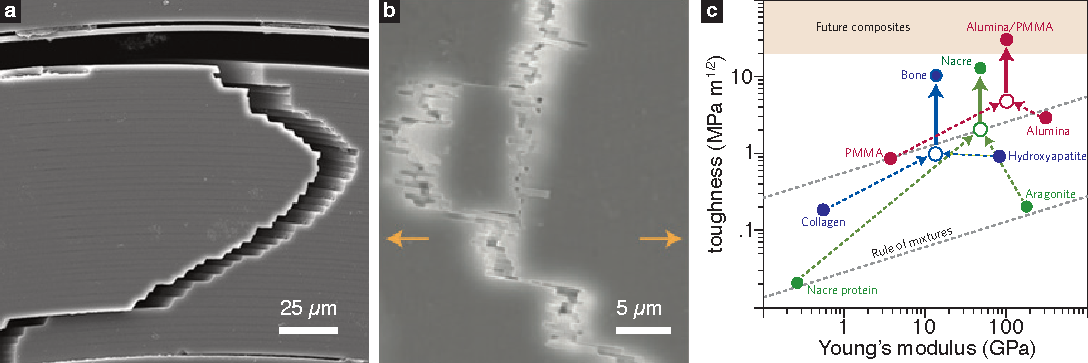
\includegraphics[width=\textwidth, trim={0 0.0cm 0.0cm 0}, clip]{Figures/Introduction/CrackPath_V2.pdf}
           \caption{ \footnotesize Complex crack paths in SBs and SB-inspired composites are responsible for toughness enhancement. (a) Cracks are deflected and split by the concentric layered architecture of a \textit{Monorhaphis Chuni} spicule (reprinted from \cite{Weaver:2010ew}). (b) Crack splitting and tablet pull-out observed during the fracture of nacre loaded in uniaxial tension (reprinted from \cite{wegst2015bioinspired}). (c) Comparison of toughness of both nacre and SB-inspired layered ceramic composites with their brittle constituents showing a toughness enhancement in excess of what is predicted by the rule of mixtures~(reprinted from \cite{wegst2015bioinspired}). The solid circles correspond to measurements of SBs and their constituents and the open circles correspond to rule of mixtures predictions.
             }
           \label{f:hyp}
    \end{figure}
%
    Our hypothesis is based on the Cook-Gordon mechanism (see Figure \ref{f:topchanges} (a))~\cite{cook1964mechanism}. This mechanism describes how a crack approaching a weak interface can become trapped and deflected along the interface, temporarily arresting the crack's growth through the material. Our hypothesis is supported by experimental observations of crack patterns in fractured SBs and SB-inspired composites (see Figures \ref{f:hyp} (a)--(b) and \ref{f:sim} (a))~\cite{barthelat2007experimental,poissant2010novel}, the PI's previous research on contact interface toughening caused by surface architectures~\cite{kesari2010role,kesari2011mechanics,kesari2011effective}, and the following two results that we obtained using a preliminary version of the regularized variational fracture theory (RVFT).

    \subsubsection{Preliminary research: 2D layered ceramic composites}

      While ceramics are lighter than metals and can withstand higher temperatures and corrosive environments, their brittleness makes them unsuitable for applications in which reliability is paramount. To make them a viable engineering material, ceramics are often made into composites. One of the simplest ceramic composite manufacturing methods is the sintered laminate technique described by Clegg et al. (see Figure \ref{f:sim} (a))~\cite{clegg1990simple} in which sheets of SiC are coated in graphite, pressed together, and sintered. While the architecture of the final composite is simple, it drastically increases the toughness of the material---i.e., the area under the load-displacement curve (see Figure~\ref{f:sim} (b)). The jaggedness seen in the load-displacement response corresponds to crack arrest and re-initiation at each of the graphite interfaces.

      Using the RVFT, the PI has explored how changing the number of layers in the 2D laminate affects its toughness (see Figure \ref{f:sim} (c)--(d)). The SiC layers were assigned a fracture initiation toughness $g_{b}$ and the graphite interfaces were assigned a lower toughness $g_{I}$. The simulations were not only able to predict crack arrest, deflection, and re-initiation at the interfaces (see Figure \ref{f:sim} (c)), but also the jagged shape of the force-displacement responses observed by Clegg et al. (see Figure \ref{f:sim} (d)). These preliminary results suggest that the RVFT is capable of predicting both the experimentally observed toughening mechanisms and the effects that small-scale architecture has on large-scale fracture behavior.
%
      \begin{figure}[h!]
             \centering
               \includegraphics[width=\textwidth, trim={0 0.0cm 0.0cm 0}, clip]{Figures/Introduction/CrackPathSim_V1.pdf}
               \caption{ \footnotesize Initial RVFT results show accurate predictions of crack paths and capture toughening mechanisms such as crack deflection in 2D composites. (a) The convoluted crack path in a 2D layered SiC/graphite composite loaded in three point bending (reprinted from \cite{clegg1990simple}). (b) The load-displacement response of the SiC/graphite composite (reprinted from \cite{clegg1990simple}). (c) Crack path predicted by the RVFT for a model of the composite shown in (a). The Young's modulus, Poisson's ratio, and the regularization parameter (see \S \ref{s:RVFTdetails}) used in the RVFT are denoted by $E$, $\nu$, and $\ell$, respectively. (d) The load-displacement response obtained from the RVFT predictions for different numbers of layers.
                 }
               \label{f:sim}
      \end{figure}

    \subsubsection{Preliminary research: fracture of wavy interfaces}

      Wavy interfaces are a prominent architectural motif in SBs, such as woodpecker beaks (see Figure~\ref{f:VFTprelimresults}~(a)), that are subject to impact or cyclic loads but must remain intact to perform their mechanical functions \cite{lee2014hierarchical, jaslow1990mechanical}.

      The PI has performed a preliminary study of crack propagation in materials with wavy interfaces using the RVFT (see Figure~\ref{f:VFTprelimresults}~(b)--(c)). In these simulations, we allowed the material's fracture initiation toughness to vary spatially, so that it had a high value, $g_{b}$, in most of the solid and a low value, $g_{I}$ at a predefined wavy interface of finite thickness. We varied the amplitude $A$ and wavelength $\lambda$ of the wavy interface and studied the effect of the ratio $A/\lambda$ on the mechanical response. We found that at small $A/\lambda$, the crack always propagated along the interface (see Figure~\ref{f:VFTprelimresults}~(c)). However, at larger $A/\lambda$ the crack repeatedly ventured from the interface into the bulk and then back into the interface through a series of energy dissipating instabilities, see Figure~\ref{f:VFTprelimresults}~(c). This process led to substantial toughening in the load-displacement response (see Figure~\ref{f:VFTprelimresults}~(b)).

      The RVFT was able to capture the crack arrest and re-initiation instability as well as the nucleation of additional daughter cracks at the crests and troughs of the wavy interface. These effects constituted the mechanisms through which the wavy interface enhanced the material's toughness.
%
      \begin{figure}[h!]
        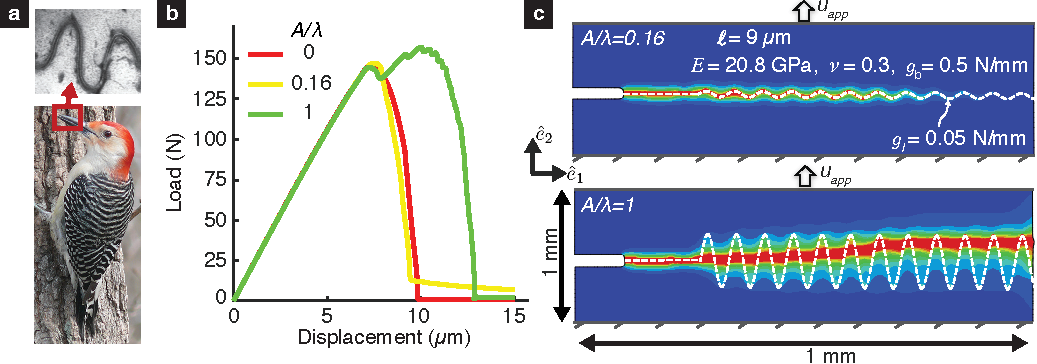
\includegraphics[width=\textwidth,trim={0 0 0 0},clip]{Figures/WavyInterface/SinusoidalInterfaceFigCrackPropagation_V8.pdf}
        \centering
        \caption{ \footnotesize (a) Wavy interfaces between keratin scales in the beak of the red bellied woodpecker (photo from \cite{birdpicture1}, micrograph reprinted from \cite{lee2014hierarchical}). (b) Load-displacement curves for different aspect ratios $A/\lambda$ of the interface shown in (c). (c) The crack propagates along the wavy interface for $A/\lambda=$0.16. However, the crack repeatedly ventures from the interface into the bulk and then back into the interface through a series of energy dissipating instabilities for $A/\lambda=$ 1. The interface is shown as a dashed line.
        }
        \label{f:VFTprelimresults}
      \end{figure}

  %%%%%%%%%%%%%%%%%%%%%%%%%%%%%%%%%%%%%%%%%%%%%%%%%%%%%%%%%%%%%%
  \subsection{Rationale underlying our research strategy}
    \label{s:rationale}
    The preliminary research discussed in \S \ref{s:hyp} shows that the evolution of crack networks and their interaction with the SB's architecture play a critical role in determining the large-scale toughness of the SB. Therefore, models that aim to quantitatively capture how small-scale architectural motifs affect large-scale toughness should incorporate, at least in some approximate manner, the evolution of crack patterns.

    The importance of the project's research objective is made evident by the plethora of theoretical solid mechanics models that have been put forth to explain the origin of toughness in SBs and SB-inspired composites~\cite{barthelat2007mechanics,smith1999molecular,meyers2008mechanical,li2004nanoscale,lin2006mechanical,chen2013bio}. As a consequence of SBs' architectural complexity, however, typical mechanics models focus on a small subset of architectural motifs and make simplifying assumptions regarding the deformation behavior of the constituent materials and the interfaces.

    Many of the existing mechanics models used to explain toughness in SBs rely on the set of toughening mechanisms originally presented by Evans \cite{evans1990perspective}. These mechanisms, such as micro cracking, fiber bridging and fiber pull-out, were first used to understand the origins of toughness in early generations of fiber reinforced composites. Similarly, the shear-lag model originally developed to describe the mechanism of force transmission in fiber reinforced composites \cite{cox1952elasticity} has also been used to explain the mechanical behavior of SBs \cite{Jackson1988,gao2003materials}. However, models based on these mechanisms fail to quantitatively capture the toughness enhancement observed in SBs \cite{barthelat2011toughness,bloyer1998fracture,wang2011deformation,nalla2005mechanistic}. This is because these models do not consider the \emph{evolution} of complex crack networks and the \emph{interaction} of the cracks with the 3D interfaces.
%
    \taburowcolors[2] 2{tableLineOne .. tableLineTwo}
      %\tabulinesep = ^4mm_3mm
      \tabulinesep = ^2mm_1mm
      \everyrow{\tabucline[.4mm  white]{}}
%
    \begin{table}[h!]
      \caption{\footnotesize A comparison of different computational fracture mechanics methods, with respect to features that are critical for pursuing the research objective.}
      \label{t:comp}
      \begin{tabu}{ X[c,3] X[c,3] X[c,2] X[c,3] X[c,4]  X[l,6] }
      \tableHeaderStyle
          CZ method (Hillerborg \textit{et al.}) & Generalized CZ method (Xu and Needleman) & Damage mechanics &  Element Deletion  & XFEM  & RVFT \\
        \multicolumn{6}{p{0.97\textwidth}}{\textbf{\textit{1. Capable of capturing topology changes independently, i.e., without  \textit{a priori} knowledge of crack path(s),  user input, or resorting to \textit{ad-hoc}, or heuristic techniques.}}}\\
               No~\cite{hillerborg1976analysis} &
               Yes~\cite{xu_1994,tijssens2000numerical}  &
               Yes~\cite{peerlings1998gradient} &
               Yes &
               No~\cite{belytschko2001arbitrary,daux2000arbitrary}&
               Yes~\cite{borden2012phase} (our preliminary research, e.g., see Figures~\ref{f:sim}, and \ref{f:xfem}) \\
                %
                %
               \multicolumn{6}{p{0.97\textwidth}}{\textbf{\textit{2. Good accuracy. Able to quantitatively reproduce experimental observations of crack growth and the evolution of a crack network as long as there are no topology changes in the network).}}}\\
              does not apply &
              No~\cite{tijssens2000numerical,de2003numerical,de2004computational} (see Figure~\ref{f:czm})&
              No  &
              No~\cite{song2008comparative} &
              competitive &
              competitive (our preliminary research, e.g., see Figure~\ref{f:VFTvalidation}) \\
              %
              %
            \multicolumn{6}{p{0.97\textwidth}}{\textbf{\textit{3. Well conditioned, i.e., no problems with numerical stablility.}}}\\
              Yes &
              Yes &
              No &
              Yes &
              No~\cite{bechet2005improved} &
              Yes~\cite{peerlings1998gradient} (our preliminary research) \\
              %
              %
              \multicolumn{6}{p{0.97\textwidth}}{\textbf{\textit{4. Mesh independence.}}}\\
               No &
               No~\cite{tijssens2000numerical,de2003numerical} &
               No~\cite{de1995comparison} &
               No~\cite{song2009cracking} &
               Yes~\cite{nicOlas1999finite} &
               Yes~\cite{miehe2010thermodynamically,bourdin2000numerical,borden2012phase} (our preliminary research) \\
               %
               %
            \multicolumn{6}{p{0.97\textwidth}}{\textbf{\textit{5. Computationally affordable.}}}\\
            Yes &
            Yes &
            No &
            Yes &
            Yes &
            No
      \end{tabu}
    \end{table}

    Even with state-of-the-art computational fracture mechanics techniques, it is challenging to accurately simulate the evolution of complex crack patterns in SBs and SB-inspired composites. We reviewed the most widely used computational fracture mechanics techniques to determine if they could be used to pursue the project's research objective. We evaluated the different techniques using five criteria that are critical for the project's success (see Table \ref{t:comp}). The generalized cohesive zone (CZ) methods, the extended finite element method (XFEM) and the RVFT came closest to satisfying the criteria, but none satisfied all five. For example, the generalized CZ method cannot accurately reproduce experimentally observed crack paths~\cite{tijssens2000numerical,de2003numerical,de2004computational}. Furthermore, the crack paths that it predicts are highly mesh sensitive. The XFEM cannot independently handle topology changes during the evolution of crack patterns. That is, it cannot capture phenomena such as the merging of two (or more) cracks to form a single crack (Figure~\ref{f:topchanges}(b)), the splitting of a crack into two (or more) daughter branches (Figure~\ref{f:topchanges}(a)), or the nucleation of new cracks (Figure~\ref{f:topchanges}(c)). Further elaboration on why the generalized CZ methods and the XFEM are not suitable for pursuing the research objective is given in \S \ref{s:extra}.
%
    \begin{figure}[h!]
          \centering
          \includegraphics[width=1.0\textwidth]{Figures/CZM/CrackPathTopology_V1MM.pdf}
          \caption{\footnotesize Examples of crack topology changes. (a) A single crack impinging on an interface (red) and branching into two cracks. (b) Two cracks propagating and merging to form a single crack. (c) The nucleation or formation of a new crack at an interface (red).}
          \label{f:topchanges}
    \end{figure}
%
    The primary drawback of the RVFT is its computational cost. Through our preliminary research we found that the RVFT's  computational cost is connected to a pathology of the theory that we call  ``crack broadening''. 
     % We explain this pathology in \S \ref{s:broadening} and 
     We propose a strategy to alleviate crack broadening so that the theory is suitable for pursuing our research objective. The proposed modification of the RVFT constitutes a new theory that we refer to as the anisotropic RVFT (aRVFT). 

%%%%%%%%%%%%%%%%%%%%%%%%%%%%%%%%%%%%%%%%%%%%%%%%%%%%%%%%%%%%%%
%%%%%%%%%%%%%%%%%%%%%%%%%%%%%%%%%%%%%%%%%%%%%%%%%%%%%%%%%%%%%%
%%%%%%%%%%%%%%%%%%%%%%%%%%%%%%%%%%%%%%%%%%%%%%%%%%%%%%%%%%%%%%
\section{Technical Background}
  %%%%%%%%%%%%%%%%%%%%%%%%%%%%%%%%%%%%%%%%%%%%%%%%%%%%%%%%%%%%%%
  \subsection{Technical details of RVFT}
    \label{s:RVFTdetails}


    A crack by definition has zero thickness in the reference configuration. Almost all  continuum mechanics fracture theories model cracks as curves or surfaces in the reference configuration. Similarly, some of the most important computational fracture mechanics methods, such as XFEM and CZ methods, also model cracks as having zero thickness~\cite{day1994zero,benvenuti2008regularized}. In contrast, a very conspicuous feature of the RVFT is that cracks have non-zero thickness. Crack networks in RVFT are represented using a scalar-valued field called the damage field. We denote the damage field as  $d(\bs{X})$, where$\bs{X}$ is a material point in the solid's reference configuration $\mathcal{B}_0$. The damage parameter $d$ takes values between zero and unity. By construction, as $d$ increases the material's capacity to store elastic energy decreases. Therefore, $d$ can be interpreted as a measure of damage. When $d=0$ the material point is completely undamaged, and when $d=1$ the material point has lost all capacity to store strain energy. The crack pattern is the region $\Omega_c$, which is defined to be a path connected subset of $\mathcal{B}_0$ such that $d(\bs{X})\ge c,~\forall\bs{X}\in \Omega_c$, where $c$ is a real number just smaller than unity, and the set $\{\bs{x}\in \Omega_c~:~d(\bs{X})=1\}$ is non-empty.

    For the sake of brevity,  we will focus on the version of RVFT presented by Bourdin et al.~\cite{bourdin2000numerical, bourdin_2008}.  That is, we do not discuss the more sophisticated versions of RVFT that include augmentations aimed at allaying unrealistic effects, such as fracture during compressive loading and healing of cracks. However, the  preliminary results shown in Figures~\ref{f:sim}, \ref{f:VFTprelimresults}, and \ref{f:VFTvalidation} were produced using the version presented by Miehe~\cite{miehe2010phase}, which contains these augmentations.

    The physics underlying Bourdin et al.'s RVFT is the variational fracture theory (VFT) put forward by Francfort and Marigo~\cite{francfort_1998}. The VFT is a generalization of the configurational force balance ideas of  Griffith~\cite{griffith1921phenomena}. Griffith postulated that for a crack to grow the energy release rate should equal or exceed the material's fracture toughness. In RVFT this postulate is generalized by requiring that the damage field only grow such that the  mechanical energy released is greater than or equal to the energy consumed by the fracture processes.  For the case of no body forces and surface tractions, this postulate implies that

    \begin{equation}
      \label{eq:PFT-Functional}
      d:=\mathrm{Arg}\inf_d
      g_c/2
      \int_{\mathcal{B}_0}
      \left(
      d(\bs{X})^2/\ell + \ell \lVert\bs{\nabla}_0d(\bs{X})\rVert^2
      \right)
      d\Omega
      +\int_{\mathcal{B}_0}
      \Psi_{d}(\mathbf{X},\bs{C}(\bs{X}), d(\bs{X}))
      %g(d(\bs{X}))\Psi_{0}(\bs{C},\bs{X})
      \, d\Omega,
    \end{equation}
    subject to the constraint that $d$ at any material point can only increase with time. This constraint introduces irreversibility and history dependence into the problem. In~\eqref{eq:PFT-Functional}, the parameter $g_c$ is a measure of the  material's fracture toughness,  $\|\cdot\|$ is the Euclidean 2-norm, the parameter $\ell$ has units of length and is called the regularization parameter, $\Psi_{d}(\mathbf{X},\bs{C}, d):=(1-d)^2 \Psi_{0}(\bs{X}, \bs{C})$ is called the degraded strain energy density,  where  $\Psi_0$ is the strain energy density of the solid when we ignore all dissipative processes. The tensor $\bs{C}:=\bs{F}^{\rm T}\bs{F}$ is the right Cauchy-Green deformation tensor, where $\bs{F}=\bs{\nabla}_{0}\bs{u}+\bs{I}$ is the deformation gradient, $\bs{u}$ is the equilibrium displacement vector, $\bs{I}$ is the identity tensor, and $\bs{\nabla}_0(\cdot)$ is the gradient operator defined with respect to $\bs{X}$.  By the  equilibrium displacement vector we mean that $\bs{u}$ satisfies the dirichlet boundary conditions and the equilibrium equation $\bs{\nabla}_0\cdot\bs{P}=0$ on $\mathcal{B}_0$, where $\bs{P}$ is the first Piola-Kirchhoff stress tensor.

    As preliminary research, we implemented nonlinear finite element techniques~\cite{belytschko2013nonlinear} to numerically solve the variational problem posed in~\eqref{eq:PFT-Functional} using the algorithms presented in \cite{borden2012phase}. The results of these calculations are shown in Figures~\ref{f:sim},~\ref{f:VFTprelimresults}, \ref{f:VFTvalidation}, and~\ref{f:xfem}. These results were generated for the special case of small deformations and $\Psi_0$ corresponding to the strain energy density of a  isotropic, linear elastic solid. We found that in many important cases the results of the RVFT match the predictions of linear elastic fracture mechanics (see Figure~\ref{f:VFTvalidation}(a)). It has  been shown that in many cases the crack paths predicted by RVFT match experimentally observed crack paths~\cite{miehe2010phase,borden2012phase,dally2015phase}. We also obtained good agreement between RVFT predictions and experimental observations of crack paths in our preliminary research (see Figures~\ref{f:sim}, \ref{f:VFTvalidation}(b), and~\ref{f:xfem}).
%
    \begin{figure}[h!]
      \centering
      \includegraphics[width=\textwidth]{Figures/VRF/Figure1_box_ver9.pdf}
      \caption{\footnotesize Comparison of RVFT predictions with LEFM and experiments. (a) Edge-notched geometry subjected to a far-field stress $\sigma^\infty$. The dimensionless stress at which the crack initiates $\sigma^\infty_{cr}/E^*$ as a function of dimensionless variables, $g_c/E^*b$ and $a/b$ obtained from the analytical solution, where $E^*=E/(1-\nu^2)$. For different values of $g_c/E^*b$, the markers lie close to the reference line shown in gray within an error of 5\% (b) Comparison of RVFT predictions with an edge notch three-point bending test in which the sample has three holes drilled in it. (i) The experimentally measured crack path from~\cite{bittencourt_1996}. (ii) Contour of the damage field $d$, where $d=1$ is indicated by red contour level signifying the location of the crack. (iii) Comparison of the measured crack path and the RVFT predictions using the crack angle, $\theta$ shown in (ii).}
      \label{f:VFTvalidation}
    \end{figure}

  %%%%%%%%%%%%%%%%%%%%%%%%%%%%%%%%%%%%%%%%%%%%%%%%%%%%%%%%%%%%%%
  \subsection{Technical problem statement: ``crack broadening''}
    \label{s:broadening}

    Cracks in RVFT are defined to be the region $\Omega_c$, and therefore have finite thickness. This does not preclude RVFT from being a useful and predictive theory of fracture (see Figures~\ref{f:sim}, \ref{f:VFTvalidation}, and~\ref{f:xfem}). However, for the cracks in RVFT to be physically meaningful their thicknesses should be much smaller than the dimensions of the solid.  This is because the crack region $\Omega_{c}$ has zero stiffness. Consequently, if a crack's thickness is not much smaller than the solid's dimensions then the failure behavior is more similar to plastic failure than brittle fracture. It is argued that the thickness of the crack is of the order of $\ell$, the regularization parameter~\cite{amiri2014phase}. By choosing $\ell$ to be much smaller than the characteristic dimension of the solid, $W$, one can ensure that the results have the physical features of brittle fracture. However, in some cases we observed that the crack thickness was comparable to the dimensions of the solid even though $\ell$ was much smaller than $W$ (see Figure \ref{f:broadening} (c)). We call this effect \textit{crack broadening}.
%
    \begin{figure}[h!]
      \centering
        \includegraphics[width=\textwidth]{Figures/Broadening/Broadening_V9.pdf}
          \caption{ \footnotesize Example simulations demonstrating the problem of crack broadening. (a) Experiment geometry and problem parameters. Only the lower half of the plate in the $\hat{\mathbf{e}}_2$ direction is shown since $d\approx 0$ in the upper half for (a)--(c). The notch is not explicitly incorporated as part of the plate's geometry but rather is represented as a small region where $d=1$, as shown in the inset. (b) The plate in (a) is loaded in uniaxial tension by displacing the boundaries marked in gray in the $\pm \hat{\mathbf{e}}_1$ direction. A crack (the red contour level) propagates from the notch in the $\hat{\mathbf{e}}_2$ direction until the plate is cleaved into two pieces. The crack's thickness is roughly equal to $\ell$. (c) The plate in (a) is loaded in uniaxial tension parallel to the notch direction by displacing the boundaries marked in gray in the $\pm \hat{\mathbf{e}}_2$ direction. Damage progresses from the notch in the $\pm \hat{\mathbf{e}}_1$ directions until there is a region of completely disintegrated material (i.e., $d\approx1$) spanning the entire width of the plate. The thickness of this region is much larger than $\ell$. (d) A 2D strip with infinite length in the $\hat{\mathbf{e}}_2$ direction stretched parallel to a crack (shown in red) along its length. (g) The variation of the damage, $d$, over the half-width of the 2D cracked strip shown in (d). The variable $\xi=x/W$, and $x$ is the Cartesian coordinate in the  $\hat{\mathbf{e}}_1$ direction shown in (d).
      }
      \label{f:broadening}
    \end{figure}
%
    We found that the crack broadening effect was due to the inadequacy of the condition $\ell/W \ll 1$. This fact is best illustrated by the following analytical solution to the variational problem~\eqref{eq:PFT-Functional} for a simple test case. Consider a 2D strip of infinite length and width $2W$ that is shown in Figure~\ref{f:broadening} (d). The strip is composed of an incompressible neo-Hookean material so that the degraded strain energy density in this case is $(1-d)^2 (\mu/2)(\lambda_1^2+\lambda_2^2-2)$. The strip has a pre-existing crack along its length (shown in red in Figure~\ref{f:broadening} (d)). The strip is uniformly stretched with a stretch ratio of $\lambda_2$ in the $\hat{\mathbf{e}}_2$ direction (see Figure~\ref{f:broadening} (d)). Let  $\tilde{\beta}:= \mu (\lambda_2^2+1/\lambda_2^2-2) W^2 /g_c  \ell$ be a dimensionless measure of this stretching, where $\mu$ is the shear modulus, and let $\tilde{\alpha}:=\tilde{\beta}+1/\tilde{\ell}^{2}$, where $\tilde{\ell}:=\ell/W$. Assuming that the solution does not vary along the strip's length, an analytical solution for the damage field can be obtained. In the majority of the strip the damage variable is approximately equal to $ \tilde{\beta}/\tilde{\alpha}$, see Figure~\ref{f:broadening} (g). If $ \tilde{\beta}/\tilde{\alpha}$ becomes greater than $c$, the parameter used for defining $\Omega_c$, then the crack width will become equal to the strip's width irrespective of how small $\tilde{\ell}$ is (see Figure~\ref{f:broadening} (g)). Therefore in order to prevent broadening, it is also necessary that $\tilde{\beta}/\tilde{\alpha}\ll 1$. In terms of dimensional variables this means $\ell \ll \ell_c$, where $\ell_c:=g_c/\mu (\lambda_2^2+1/\lambda_2^2-2)$ is a length scale characteristic of the material and loading.

    This preliminary research has an important consequence. From a practical perspective, the computational cost grows inversely with $\ell$.  Therefore, one would like to use as large an $\ell$ as possible.  However, a $\mathit{\Gamma}$ convergence~\cite{braides2002gamma} proof given in~\cite{chambolle_2005, ambrosio_1990b} shows that the RVFT solutions are only physically meaningful in the limit $\ell\to 0$. The proof unfortunately does not tell us what is the largest value of $\ell$ for which the results are still useful. Our analysis answers this question by stating that $\ell$ should be smaller than $\rm{min}\{W, \ell_c\}$.

    While it might appear that the solution to the broadening problem is straightforward---simply make $\ell$ smaller than both $W$ and $\ell_c$---this is much easier said than done. For most practical applications, the value for $\ell_c$ is so small that using $\ell$ values smaller than $\ell_c$ is impractical in terms of computational cost. For example, $\ell_c\approx 10\unit{nm}$ for silicon. In this case, even a 2D, $1\unit{\mu m}$ square specimen would require solving one million equations.  Thanks to recent advances in parallelization and computational power, solving 0.3 million equations takes us roughly 900 CPU core hours. However, pursuing the project's research objective requires us to run a RVFT simulation repeatedly to study the effect of different architectural motifs on an SB's toughness.

    In summary, crack broadening is a major problem, and because of it computational simulations based on the current RVFT cannot be used as practical investigative tools. However, by reformulating RVFT to eliminate the crack broadening problem, much larger $\ell$ values could be used, drastically reducing the computational cost and making this method viable as an investigative tool.

%%%%%%%%%%%%%%%%%%%%%%%%%%%%%%%%%%%%%%%%%%%%%%%%%%%%%%%%%%%%%%
%%%%%%%%%%%%%%%%%%%%%%%%%%%%%%%%%%%%%%%%%%%%%%%%%%%%%%%%%%%%%%
%%%%%%%%%%%%%%%%%%%%%%%%%%%%%%%%%%%%%%%%%%%%%%%%%%%%%%%%%%%%%%
\section{Proposed research: aims and tasks}
    \label{s:aims}
    We will pursue the project's overarching  research objective by pursuing the following two specific aims and carrying out their associated tasks.

    % \begin{description}
    %   \item[Aim 1 (A1):] We will develop a new variational fracture theory and computational framework that are capable of robustly simulating crack topology changes (crack branching, merging, etc.) in composites with complex, 3D architectures and heterogeneities.
    %   \begin{description}
    %     \item[Task Aim 1 Task 1] \textit{Develop a new RVFT  that will be free of the problem of crack broadening. We call this new RVFT the anisotropic RVFT or aRVFT.}
    %     \item[Task Aim 1 Task 2] \textit{Develop new computational tools by using nonlinear finite element techniques  to numerically solve the aRVFT.}
    %     \item[Task Aim 1 Task 3] Simulate well studied linear elastic fracture mechanics problems and experimental  fracture tests using the aRVFT computational tools developed in Aim 1 Task 2. Ensure that crack broadening has been eliminated in the aRVFT computational tools, and that they are more computationally affordable than those based on the current RVFT.
    %   \end{description}
    %
    %   \item[Aim 2 (A2):] If the new RVFT is to function as an investigative tool for identifying the key architectural features, then it is important that it can reproduce the salient features of the experimentally observed failure responses of composites. We will use the aRVFT computational tools to simulate the failure of a model SB---spicules from the marine sponge \textit{Euplectella aspergillum}.
    %   \begin{description}
    %     \item[Task Aim 2 Task 1] Build an aRVFT computational model for the spicule. In order to build an aRVFT model of a spicule we must first characterize the spicule's architecture and measure the mechanical properties of its constituent material and the interfaces within it.
    %     \item[Task Aim 2 Task 2] Characterize the spicules' failure behavior by performing three-point bending tests on notched spicules.
    %     \item[Task Aim 2 Task 3] Compare the results from the aRVFT simulation performed in Aim 2 Task 1 with measurements from fracture tests performed in Aim 2 Task 2. Evaluate whether the aRVFT was able to capture the spicule's failure behavior by using the load-displacement responses as well as the work of fracture as comparison metrics.
    %   \end{description}
    % \end{description}

  %%%%%%%%%%%%%%%%%%%%%%%%%%%%%%%%%%%%%%%%%%%%%%%%%%%%%%%%%%%%%%
  \subsection{Aim 1: Develop a new variational fracture theory and computational framework that are capable of robustly simulating crack topology changes}
   \label{s:A1}

   Through our preliminary research, we have developed a promising strategy to eliminate crack broadening.  In the current RVFT, the material's stiffness is uniformly degraded in all directions as $d$ increases. We illustrate this situation schematically in Figure~\ref{f:broadening} (e), where bonds both perpendicular and parallel to the crack are broken. Physically, however, it is only necessary that bonds perpendicular to the crack are broken (see Figure~\ref{f:broadening} (f)). We found that the artificial degradation of bonds parallel to the crack causes crack broadening in the current RVFT. Therefore, we will solve the problem of crack broadening by developing a new RVFT in which the parallel bonds are not broken. Due to the anisotropic breaking of bonds, we refer to our new RVFT as anisotropic RVFT, or aRVFT. In aRVFT, we will introduce information about the crack orientation and use that information to only degrade the stiffness in the direction normal to the crack surface. Specifically, we will make the strain energy term in ~\eqref{eq:PFT-Functional} have the more general form $\int_{\mathcal{B}_0}\mathsf{\Psi}(\bs{X}, \bs{F},\hat{\bs{D}},d)\, d\Omega$, where $\hat{\bs{D}}$ is a unit vector containing information about the orientation of the crack. If $d=1$ at some $\bs{X}_c$ and there is a single crack containing $\bs{X}_c$, then $\hat{\bs{D}}(\bs{X}_c)$ is normal to that crack at that point. Using $\hat{\bs{D}}$ we will construct $\mathsf{\Psi}$ so that the stiffness is only degraded in the direction normal to the crack. Our preliminary calculations below show that this strategy is promising for resolving the problem of broadening.

   \subsubsection{Aim 1 Task 1: Develop a  new RVFT that will be free of the problem of crack broadening}
    The construction of $\mathsf{\Psi}$ may appear challenging.  However, it can be simplified by making use of the fact that any proposed $\mathsf{\Psi}$ has to satisfy the fundamental principles of material behavior and mechanics.  For example, we will reduce the allowable forms of $\mathsf{\Psi}$ by requiring that it obeys the principle of material frame indifference, and respects the symmetries of the material. We found that for an isotropic material ${\mathsf{\Psi}}$ satisfies these conditions if it has the reduced form ${\mathsf{\Psi}}(\bs{X}, \hat{\bs{D}}\cdot\mathbf{A}(\bs{U})\hat{\bs{D}}, \lambda_1, \lambda_2,\lambda_3)$, where $\bs{U}$ is the positive square root of $\bs{C}$, $(\lambda_1,\lambda_2,\lambda_3)$ are the eigenvalues of $\bs{U}$, and the tensor valued function $\bs{A}(\bs{U})$ satisfies the condition $\bs{A}(\bs{Q}\bs{U}\bs{Q}^{\text{T}})=\bs{Q}\bs{A}(\bs{U})\bs{Q}^{\text{T}}$.  In 2D consider $\mathsf{\Psi}_d^{\text{NH}}=\mu/2((\lambda_1^2+\lambda_2^2-2)-d( a_1^2\lambda_1^2+a_2^2\lambda_2^2-1))$, where $a_1$, $a_2$ are the components of $\hat{\bs{D}}$ in the eigenvector directions of $\bs{U}$.  This strain energy density function is a specialization of the reduced form for the case $\bs{A}(\bs{U})=\bs{U}^2$. When $d=0$ everywhere then it reduces to the classical incompressible neo-Hookean material model.


    If we re-solve the 2D cracked strip problem (see Figure~\ref{f:broadening} (d)) using $\mathsf{\Psi}_d^{\text{NH}}$ instead of the previously used $(1-d)^2 (\mu/2)(\lambda_1^2+\lambda_2^2-2)$, we find that if $\ell \ll W$, then at distances of the order $\ell$ away from the pre-existing crack, $d(\xi)<  2e^{-1/\tilde{\ell}}+O(e^{-2/\tilde{\ell}})\approx 0$ irrespective of the amount of stretch $\lambda_2$ or the value of $\mu$. Thus, with the new $\mathsf{\Psi}_d^{\text{NH}}$, the broadening effect has vanished. These results give us confidence that by reformulating RVFT we can eliminate the issue of crack broadening.

    As the logical next step, we will confirm that the proposed $\mathsf{\Psi}_d^{\text{NH}}$ eliminates broadening by analytically solving problems with more complex stress states than that shown in Figure~\ref{f:broadening} (d). Using $\mathsf{\Psi}_d^{\text{NH}}$ as guidance,  we will then derive a family of degraded strain energy density functions that eliminate broadening for 3D, compressible, and heterogeneous solids. We will derive the nonlinear partial differential equation (PDE) that $d$ must satisfy for it to be the solution to the variational problem~\eqref{eq:PFT-Functional} for progressively more complex situations. For example, we will move from small  to finite deformations, homogenous to heterogenous solids, 2D to 3D geometry, and quasi-static to dynamic.

   \subsubsection{Aim 1 Task 2: Numerically implement aRVFT}
    We will numerically implement the new aRVFT using the same finite element techniques and nonlinear solver algorithms that we used for producing the preliminary results shown in Figures~\ref{f:sim}, \ref{f:VFTvalidation}, and \ref{f:xfem}.  The numerical implementation will progress from simple versions of the aRVFT to  progressively more complex versions.  For example, we will first implement a 2D version and then a 3D version.  Similarly, we will first implement the aRVFT for the case of small deformations and later for finite deformations.   To simulate quasitatic loading, we will use the nonlinear solver algorithms used in~\cite{miehe2010phase}. For simulating dynamics, we  will use the time integration algorithms used in~\cite{borden2012phase}. In the final stages, we will implement the augmentations used by Miehe~\cite{miehe2010phase} to prevent the damage field from ever decreasing with either   load-step (in quasistatic simulations) or time (in dynamic simulations). This augmentation guarantees irreversibility of crack growth. We will use the techniques described in ~\cite{miehe2010phase}  to  avoid the spurious effect of the damage variable growing  when the stress state is purely compressive.

  \subsubsection{Aim 1 Task 3: Simulate well studied linear elastic fracture mechanics problems and well known  experimental  fracture tests using the  computational tools developed in Aim 1 Task 2.}
    We will simulate the  fracture mechanics problems and experimental tests shown in Figs.~\ref{f:sim}, \ref{f:VFTvalidation},  and \ref{f:xfem} using the  computational tools developed via Aim 1 Task 2.
    We will use these simulations to ensure that broadening has  been eliminated in the newly developed computational tools and that the  simulations performed using  these tools are more computationally affordable than those based on the current RVFT.

  %%%%%%%%%%%%%%%%%%%%%%%%%%%%%%%%%%%%%%%%%%%%%%%%%%%%%%%%%%%%%%
  \subsection{Aim 2: Evaluate the predictive potential of the aRVFT through experimental comparison}
    \label{s:A2}

    Once free of crack broadening, the aRVFT-based computational tools will be able to model the evolution of complex fracture patterns in realistic models of composites with complex architectures.
    %
    The goal of developing the aRVFT is to use it for performing accurate and robust virtual experiments on SBs and SB-inspired composites.
    %
    However, to realize this goal it is important that the aRVFT tools are able to correctly capture the salient characteristics of a composite's failure behavior. We will evaluate the predictive capability of the developed aRVFT tools by comparing their results with measurements from fracture tests conducted on a model SB with 3D architecture.

    We will use the skeletal elements of the marine sponge \textit{Euplectella aspergillum}, called spicules, as the model SB in our evaluation~\cite{mayer2004lessons,sarikaya2001biomimetic}.
    %
    The \textit{E. aspergillum} spicules are hair-like fibers that are roughly 10 cm long and 50 $\mu$m in diameter and are composed primarily of silica.
    %
    They have a tubular, tree-ring type architecture (see Figure~\ref{f:exp} (a)), and our preliminary mechanical tests suggest that the interfaces between adjacent silica cylinders are weak.
    %
    The PI has considerable experience studying structure-property connections in spicules~\cite{monn2015new,monn2017enhanced,monn2017new}.
    %
    However, the primary reason for selecting \textit{E. aspergillum} spicules over other SBs, such as shell or bone, is that their architecture has a good balance between mathematical regularity and complexity.
    %
     Owing to their axisymmetry, the \textit{E. aspergillum} spicules can be described using less than 30 parameters.
    %
    This will allow us to build computer aided design (CAD) models of the spicules and complete our evaluation within the allocated time period of the project.
    %
    Furthermore, our preliminary mechanical tests show that the \textit{E. aspergillum} spicules' failure response is considerably different from that of spicules from a related species that lack the tree-ring architecture \cite{monn2017enhanced}.
    %
    This implies that there are interesting architecture-based toughening mechanisms operating in \textit{E. aspergillum} spicules.

    \subsubsection{Aim 2 Task 1:  Build an aRVFT computational model for the spicule}
      To build an aRVFT computational model of the spicule, we need the following information: spicule architectural parameters,
      %
      elastic and fracture toughness properties of the spicule's silica,
      %
      and fracture toughness of the spicule's interfaces.
      %
      This data will be collected through the following subtasks:

      {\fontfamily{phv}\fontseries{bc}\selectfont Task 1.i}) \textit{Measure architecture}.
        The PI has used SEM imaging to measure the silica cylinder thicknesses in the \textit{E. aspergillum} spicules as reported in ~\cite{monn2015new}.
        %
        We will measure the spicule radius, core radius, and silica cylinder thicknesses using the procedure described in~\cite{monn2015new} for all spicules that we test in Task 2.

      {\fontfamily{phv}\fontseries{bc}\selectfont Task 1.ii}) \textit{Measure fracture toughness and elastic modulus of the spicule's biogenic silica.}
        Although the \textit{E. aspergillum} spicules are predominantly composed of silica, it has been shown that many spicules from other sponge species  possess a proteinaceous scaffold within their silica~\cite{wang2010morphology, weaver2003nanostructural}.
        %
        Therefore, we will measure the elastic modulus and toughness of the \textit{E. aspergillum} spicules' silica using nanoindentation. The toughness properties of the silica cylinders in the spicules of the sponge \textit{Monorhaphis chuni} have previously been measured using nanoindentation~\cite{woesz2006micromechanical, Miserez:2008wf}. We will use the same experimental protocol in our work.
        %
        The spicule's core is roughly 20 $\mu$m in diameter, which is a sufficient area for performing the nanoindentation tests. We will compute the silica's toughness using the classic Lawn-Evans-Marshall model~\cite{lawn1975indentation, evans1976fracture}. Nanoindentation will also be used for measuring the silica's reduced elastic modulus, $E^*$. For that purpose we will follow the procedure described in~\cite{oliver1992improved}. The PI has previous experience measuring mechanical properties using nanoindentation~\cite{kesari2010role, kesari2011mechanics}.

      {\fontfamily{phv}\fontseries{bc}\selectfont Task 1.iii}) \textit{Measure the fracture toughness of spicules' interfaces.}
        Since the spicules' silica cylinders are both thin and brittle, measuring the fracture toughness, $g_{I}$, of the weak interfaces between them is a challenging task. Motivated by the classical fiber push-out test~\cite{marshall1984indentation}, which is used to measure interface toughness in fiber reinforced composites, we have designed the following ``cylinder push-out'' test for measuring $g_{I}$.

        One broken spicule segment from each bending test (see Task.2) will be embedded in epoxy and cross-sectioned using a diamond saw to create a 1--3 mm thick slab (see Figure~\ref{f:exp} (e)).
        %
        The exposed spicule cross-section will first be polished, and then a blunt diamond indenter will be used to push against the core.
        %
        On the opposite side of the slab, all silica cylinders will be mechanically supported (see Figure~\ref{f:exp} (e)).
        %
        \begin{figure}[h!]
          \centering
            \includegraphics[width=\textwidth]{Figures/spicule/Layer_spicule_ver11.pdf}
            \caption{\footnotesize Measurement of the mechanical properties and behavior of spicules. (a) A SEM image of a \textit{E. aspergillum} spicule's cross-section showing its layered architecture. The scale bar measures 10 $\mu$m. (b) The three-point bending configuration used for the fracture tests described in Aim 2 Task 2. The spicule is encastered at both ends with epoxy. A wedge-like indenter applies a force $F$ midway along the spicule's length perpendicular to its axis. (c) SEM micrograph of a notch cut in a spicule using focused ion beam milling. The scale bar measures 500 nm. (d) The load $F$ and load line displacement $w_0$ from a notched spicule (shown schematically in (b)). (e) Configuration of the the proposed cylinder push-out test. A spicule is embedded in epoxy, and cross-sectioned along the orange planes. The silica cylinders from the cross-section are mechanically supported from below and the core is pushed from above (shown in gray). The light blue lines indicate the interfaces between silica cylinders and between the first cylinder and the core. The initial interface crack with length $l_d$ is marked. (f) A typical load-displacement response obtained from a fiber push-out test (data obtained from~\cite{bright1989interfacial}).}
            \label{f:exp}
        \end{figure}
        %
        This configuration will block the relative motion of all weak interfaces except the first between the core and its adjacent silica cylinder.
        %
        Thus, the core and the silica cylinders are analogous to the fiber and matrix, respectively, in a fiber push-out test~\cite{marshall1984indentation}.

        We will adapt the mechanical testing system, which we use to perform bending tests (Aim 2 Task 2) to perform the cylinder push-out tests. During the tests we will measure the applied force and indenter displacement.
        %
        We have made preliminary estimates of the force and displacement ranges needed for this test and found that our modified testing system will be able to perform the cylinder push-out test with 50 nm displacement resolution and 4 $\mu$N force resolution.

        A typical load-displacement curve from a fiber push-out test performed on a silicon carbide fiber reinforced composite is shown in Figure~\ref{f:exp} (f).
        %
        Initially, the applied force increases linearly with indenter displacement.
        %
        The abrupt drop in force from $P_d$ to $P_d^\prime$ corresponds to the formation of a crack along the fiber-matrix interface shown schematically in Figure~\ref{f:exp} (e).
        %
        Upon further loading, the  applied force again increases until it reaches $P_i$, at which point the crack begins to propagate along the length of the fiber.
        %
        If the length of the crack $l_d$ at $P_d^\prime$ is large compared to the core radius, $r_0$, then the initiation force, $P_i$, is related to $g_{I}$ as $P_i=2\pi \sqrt{r_0^3 g_{cI} E^*}$~\cite{outwater1970fracture, kerans1991theoretical, liang1993mechanics}.
        %
        Knowing $E^*$ (from Task 1.ii) and $r_0$ (from Task 1.i), we can then compute $g_{I}$ by measuring $P_i$ in the cylinder push-out test. However, we must verify that $l_d \gg r_0$.
        %
        We can compute $l_d$ by measuring the stiffness from the force-displacement response before and after crack nucleation and choosing $l_d$ in a finite element model to match this stiffness ratio.
        %
        If $l_d$ is not much larger than $r_0$, then we will numerically compute the energy release rate for the cylinder push-out test using a finite element model in order to obtain $g_I$~\cite{moran1987crack}.

    \subsubsection{Aim 2 Task 2: Characterize the spicules' failure behavior}
      We will characterize the spicules' failure behavior by measuring the load-displacement response of a notched spicule in a three-point bending fracture test.
      %
      The PI has designed and built a mechanical testing system that is capable of performing the fracture tests with 200 nm displacement resolution and 20 $\mu$N force resolution \cite{monn2017enhanced,monn2017JoVE}. The system's design is based on that of an Atomic Force Microscope (AFM). The PI has considerable experience using AFMs for performing mechanical tests~\cite{kesari2010role,kesari2011mechanics} and has also performed three-point bending tests on spicules without notches using the custom-built system \cite{monn2017enhanced,monn2017JoVE,monn2017new}.
      %
      In the proposed tests, we will cut notches in the spicules in order to match the initial damaged state of the spicules in our simulations. Through our preliminary research we were able to successfully create 5--25 $\mu$m long notches with a sharpness of approximately 100 nm using focused ion beam (FIB) milling (see Figure~\ref{f:exp} (c)).

      Preliminary results from a bending fracture test performed on a notched spicule are shown in Figure~\ref{f:exp} (d). The applied force $F$ and load-line displacement $w_0$ are measured as the spicule is loaded in the configuration shown in Figure~\ref{f:exp} (b). The spicule is first loaded (yellow points) until a crack emanating from the notch root propagates completely across the spicule's cross-section. The spicule is then unloaded (blue points), and the area between the loading an unloading branches constitutes the total energy dissipated by the fracture process.

    \subsubsection{Aim 2 Task 3: Compare the measurements to the aRVFT tool's predictions}
      We have designed the experiments and simulations so that the geometry, internal architecture, initial damage condition, and material properties match as closely as possible. Thus, we can characterize the aRVFT's predictive capability by whether it is able to reproduce the measured load-displacement curves. Based on statistics from our initial un-notched bending measurements, we plan on testing 60 spicules harvested from four different \textit{E. aspergillum} skeletons.
%
      \begin{table}[H]
        \center
        \caption{Project timeline}
        \label{t:timeline}
        \rowcolors{1}{lightgray}{white}
        \begin{tabular}{clll}
          \hline
          Aim\textbackslash Year & 1 &  2 &  3 \\
          \hline
          Aim 1 & Task 1 & Task 2, Task 3 &  \\
          Aim 2 & Task 1.i, Task 2 & Task 1.ii & Task 1.iii, Task3 \\
          \hline
        \end{tabular}
      \end{table}

%%%%%%%%%%%%%%%%%%%%%%%%%%%%%%%%%%%%%%%%%%%%%%%%%%%%%%%%%%%%%%
%%%%%%%%%%%%%%%%%%%%%%%%%%%%%%%%%%%%%%%%%%%%%%%%%%%%%%%%%%%%%%
%%%%%%%%%%%%%%%%%%%%%%%%%%%%%%%%%%%%%%%%%%%%%%%%%%%%%%%%%%%%%%
\section{Broader impacts of the proposed work}
  \label{s:broaderimp}
  \paragraph{Collaboration with the SciToons initiative}
    The Science Cartoons (SciToons) initiative is a new strategy for communicating scientific research and concepts to a broad audience via storytelling, animation, high-quality multimedia and art. The initiative, part of broader impacts and education activities at Brown University's Science Center, engages STEM students, non-STEM students and faculty to create science animation videos that conceptualize and communicate science in an engaging manner to a broad range of audiences. The PI and his students will collaborate with the SciToons Creation Group led by Dr. Oludurotimi Adetunji, Associate Dean for Undergraduate Research and Inclusive Science; and Executive Producer of the Brown University SciToons Initiative. The SciToons Creation Group consists of both STEM and non-STEM students, STEM domain content experts, voice over artists and animators.

    The SciToons program's broader impacts goal of fostering greater understanding and appreciation of science in the general public is advanced by meshing communication and science, skills and interests of STEM and non-STEM majors. The PI and one of his current students have collaborated with Dr. Adetunji to produce a SciToon animation that, through jargon-free language and storytelling, communicates the importance and impact of the results from the PI's recent publication~\cite{monn2015new} to a non-scientific audience~\cite{ScitoonsPNAS}. As part of the proposed project, the PI, in collaboration with SciToons, will create one video per academic year for the next three years. The collaboration through this proposal will begin in Fall 2018. The videos will focus on the latest results from the research wing of the project. They will end by highlighting that the vast majority of the nature's designs are still unknown, and we will try to excite the viewers about the immense possibilities that the discovery of such designs would create for science and engineering. Funds to support the PI's future collaboration with the SciToons initiative are requested as part of the budget (see Budget Justification). \emph{Evaluation}: The viewing impact of each SciToons video is gauged by the number and geographic distribution of views the videos generate on google analytics data. Prior SciToons videos have been viewed in over 180 countries. Examples of completed SciToons can be viewed on the SciToons' YouTube channel.

    In addition to the SciToons YouTube channel and dedicated website, the videos are distributed via a variety of social media platforms, such as Twitter (@Sci\_Toons) and Facebook. The SciToons videos will also be posted on the PI's lab website. The website will be set up so that viewers can post comments and questions about the videos. The PI and his students will host a monthly virtual discussion group on Google Hangouts and address the posted comments and questions live. The PI will use the SciToons videos in the undergraduate courses he teaches at Brown, such as Advanced Engineering Mechanics (ENGN 1370) and Advanced Engineering Optimization (ENGN 1950), which share the elements of solid and structural mechanics, and optimization principles with the topics that will be highlighted in the videos. The PI will also encourage his colleagues at Brown and other universities to use the videos in introductory engineering courses and in courses related to mechanics and optimization. \emph{Evaluation}: The videos' impact and utility in the classroom with be gauged by using the end of course student feedback form.

  \paragraph{Collaboration with Spira}
    Spira is a four week camp hosted at Brown every summer for high school age girls to explore engineering. For the past four years, the PI and his students have been collaborating with Spira in order to encourage young women to pursue education in STEM fields by exposing them to interesting applications of engineering. The camp is free to those who attend and often attracts students from underrepresented minorities.  Over the course of the proposed project, every summer, the PI and the students associated with the project will design and organize talks, workshops and competitions for the Spira participants. These activities will be tailored to make the participants aware of the wide range of exciting opportunities that are only recently becoming available to engineers, and through this awareness attract them to science and engineering. \emph{Talks:} Some of the past talks have been  ``Better materials through micro-scale mechanical design'' and ``Bio-inspired engineering: why should we listen to nature.'' These talks were focused on the importance of bio-inspired materials to the future of mechanical engineering. Future talks will have a similar focus. The new results from the research component of the project will be used to enhance the quality of the talks. Following the talk, the students will be given a tour of PI's lab during which the presented research will be further explained using practical demonstrations. \emph{Lab tour and workshop:} During the lab tour, the PI and his students will also explain the operating principles behind the different lab equipment. Last year's workshop was titled, "Hidden genius: a closer look at nature's architecture.'' In it, the participants examined spicules from the \textit{E. aspergillum} sponge as well as other biomaterials. The first workshop that will be held as part of the project is tentatively titled, ``Engineering Principles in Nature''.  In it, the PI's team and the participants will discuss the size, form, and function relationships in SBs, such as mammalian bones, eggshells, gecko's feet and the venus fly trap. \emph{Competition:} The competitions will give the participants an opportunity to learn through hands-on practice and experimentation. A competition under development for this project's Spira activities is tentatively titled ``Soft landing: better materials for tomorrow's helmets and cars''. In the competition the participants will be asked to construct a structure for cushioning the fall of a dropped egg by taking inspiration from nature. The student teams will be supplied with various materials and given access to the microscope in the PI's lab. Funds to organize this new competition in collaboration with Spira are requested as part of the budget (see Budget Justification). \emph{Evaluation:} The effectiveness of the planned Spira lectures, tutorials, and competitions will be gauged using exit interviews. The students' feedback will also be solicited by encouraging them to post comments and suggestions on the Spira section of the PI's website.

%%%%%%%%%%%%%%%%%%%%%%%%%%%%%%%%%%%%%%%%%%%%%%%%%%%%%%%%%%%%%%
%%%%%%%%%%%%%%%%%%%%%%%%%%%%%%%%%%%%%%%%%%%%%%%%%%%%%%%%%%%%%%
%%%%%%%%%%%%%%%%%%%%%%%%%%%%%%%%%%%%%%%%%%%%%%%%%%%%%%%%%%%%%%
\section{Results from prior NSF support}
  \label{s:priorfund}
  CMMI-1562656: ``Emergence of New Properties at the Large-Scale on Elastic Surfaces due to  Small-Scale Adhesion and Waviness,'' \$375,000, 03/01/2016 -- 02/28/2019. \textbf{Intellectual merit} The objective of this research is to understand how contact interactions between two surfaces at the micro-scale manifest as friction-like behavior at the macro-scale. Specifically, we relate friction at the macro-scale to dissipative mechanisms acting at the micro-scale that are activated by both adhesion and surface roughness. Through a synergistic combination of theoretical analysis, computer modeling, and experiments we will develop a rigorous mechanical theory governing the relationship between friction, adhesion, and surface roughness. A better understanding of this relationship could lead to advances in pick-and-place technology, microelectromechanical systems, and biomimetic climbing robots. Four peer reviewed journal articles have been produced under this award so far~\cite{monn2017new,monn2017enhanced,monn2017JoVE,deng2017molecular}, and three others are currently in preparation. Additionally, results from these articles have been disseminated through six conference presentations. As per the Data Management Plan for this award, computer code, experimental data, and theoretical results are made available through the Dropbox cloud storage system. \textbf{Broader impacts} Five graduate students (Wenqiang Fang, Weilin Deng, Michael Monn, Jarod Ferreira, Jianzhe Yang), and one undergraduate student (Christopher Owen-Elia) have worked on projects supported by this award. Two masters theses titled ``Adhesive contact experiments with nonlinear model fitting''  and ``Deep indentation contact experiments with nonlinear model fitting'' have been completed by Jarod Ferreira and Jianzhe Yang, respectively, under the supervision of the PI. Finally, the PI has worked with the SciToons initiative at Brown University to create the first of a series of animated videos with a focus on bio-inspired engineering. The PI's collaboration with SciToons will be used to communicate research results to the STEM-interested public.

%%%%%%%%%%%%%%%%%%%%%%%%%%%%%%%%%%%%%%%%%%%%%%%%%%%%%%%%%%%%%%
%%%%%%%%%%%%%%%%%%%%%%%%%%%%%%%%%%%%%%%%%%%%%%%%%%%%%%%%%%%%%%
%%%%%%%%%%%%%%%%%%%%%%%%%%%%%%%%%%%%%%%%%%%%%%%%%%%%%%%%%%%%%%
\section{Additional details: evaluating suitability of CZ methods and XFEM for pursuing the research objective}
  \label{s:extra}
  %%%%%%%%%%%%%%%%%%%%%%%%%%%%%%%%%%%%%%%%%%%%%%%%%%%%%%%%%%%%%%
  \subsection{Cohesive zone methods}
    \label{s:CZM}
    Cohesive zone (CZ) methods have proven to be very significant for modeling interfacial fracture. These methods are based on the work of Dugdale \cite{dugdale1960yielding} and Barenblatt \cite{barenblatt1962mathematical} and built atop of classical finite elements techniques. Crack growth is modeled by allowing adjacent finite element pairs to separate along their shared boundary. As the elements separate, tractions are applied on the separating element faces as per a pre-assigned traction-separation law. The shape of and parameters in the traction-separation law can be chosen to model different types of damage behavior (ductile, quasi-brittle, etc.). This idea is made numerically feasible by incorporating what are called \textit{cohesive zone elements} between the shared boundaries of the adjacent finite element pairs. The CZ methods can be divided into two primary classes, whose difference lies in the selection of the finite element boundaries at which the CZ elements are included.

    In the classical version of the CZ method, given by Hillerborg et al., the CZ elements are only placed along element boundaries that are known or expected to be close to the final crack path \cite{hillerborg1976analysis}. This requires some \textit{a priori} knowledge of the crack path. Since the success of the proposed research project hinges on the ability to predict the evolution of complicated crack paths for which we have little to no \textit{a priori} knowledge, classical CZ methods are not suitable for the proposed research project.

    In the generalized version presented by Xu and Needleman, the CZ elements are placed between all shared element boundaries~\cite{xu_1994,camacho1996computational}. This enables the simulation of crack propagation without \textit{a priori} knowledge of the crack path. This  generalized version is also capable of modeling the evolution of complicated crack paths. However, based on our study of the computational mechanics literature and our preliminary research we found that the  generalized CZ method does not accurately reproduce experimentally observed crack paths~\cite{tijssens2000numerical,de2003numerical,de2004computational}. For example,  Figure~\ref{f:czm} shows a comparison between  experimentally observed crack paths and those that were predicted using the generalized CZ method. Furthermore, as can be seen from Figure~\ref{f:czm}(b)--(c), the crack paths predicted by the generalized CZ method are \textit{mesh dependent}. That is, they depend on the size and structure of the finite element mesh.

    The inaccuracy and  mesh sensitivity of the generalized CZ method is widely discussed in literature \cite{de2003numerical,de2004computational,tijssens2000numerical,song2008comparative}. We do not have any ideas regarding how to remedy these major problems. Therefore, we decided not to use CZ methods to pursue the project's research objective.
%
    \begin{figure}[h!]
          \centering
          \includegraphics[width=\textwidth]{Figures/CZM/CZM_crack_path_ver3.pdf}
          \caption{\footnotesize Comparison between experimentally observed and computationally predicted crack paths. (a) shows the experimental crack paths observed in concrete specimens by Schlangen~\cite{schlangen1993experimental} and the corresponding experimental setup is shown in the inset, which is a single edge notch (SEN) shear load test. Each curve corresponds to a different specimen. (b) and (c) show the computationally predicted crack paths for a coarse and fine finite  element mesh, respectively. These computational crack paths  were predicted by Tijssens\textit{et al.}~\cite{tijssens2000numerical} for the experiments shown in (a) using the generalized CZ method.}
          \label{f:czm}
    \end{figure}

  %%%%%%%%%%%%%%%%%%%%%%%%%%%%%%%%%%%%%%%%%%%%%%%%%%%%%%%%%%%%%%
  \subsection{Extended Finite Element methods (XFEM)}
    \label{s:XFEM}
    \begin{figure}[h]
      \centering
      \includegraphics[width=\textwidth]{Figures/XFEM/concrete_ver4.pdf}
      \caption{\footnotesize Comparison between experimentally observed and computationally predicted crack paths. (a) shows a photograph of a failed concrete specimen. This is from the experiments reported by G{\'a}lvez \textit{et al.}~\cite{galvez1999fracture}.   The specimen was prepared by  cutting two notches, one  on each of its   left and right edges.  The only loading on the specimen was on its  top portion. That is,   the region above the notches was loaded in compression. The specimen was observed to fail through the formation and  propagation of two distinct crack systems.  The first system   (marked as a yellow region)  consists  of two cracks, each of which  emanates  from a  notch and  grows a short distance into the  bottom portion of the specimen. The second system (marked as a red region) consists  of a single crack that nucleates in the top portion of the specimen and propagates symmetrically towards the left and right.  (b) shows the predictions of the RVFT.  As can be seen, the RVFT captures both system 1 and 2 of the cracks formed. Its predicted shape and length of the  system 1 cracks is also quite consistent with what is experimentally observed.  Its  predicted shape and length of the system 2 crack is  slightly different from what is observed in experiments. We believe that this disparity is due to the incomplete knowledge we have about the specimen's materials properties and the experiment's loading program. (c) shows the predictions from the XFEM (as implemented in Abaqus). The XFEM is able to capture the system 1 cracks. However, it completely misses the  system 2 cracks. This is expected, since as we discuss in the text, XFEM on its own cannot readily capture  topology changes, of which crack nucleation is a special case. Also, the XFEM predicted length of the  system 1 cracks is substantially  different from what is observed experimentally. }
      \label{f:xfem}
    \end{figure}
%
    The XFEM has been used to  simulate quasi-static crack growth in both 2D~\cite{belytschko1999elastic,bordas2007extended,dolbow_1999} and 3D~\cite{sukumar2000extended,moes2002non,gravouil2002non}, and dynamic crack growth in 2D~\cite{belytschko2003dynamic,song2006method}. It is currently widely used to predict crack paths~\cite{golewski2012numerical,barkai2012crack,peng2017extended} and is even a feature in commercial finite element software packages like Abaqus~\cite{abaqus2014}. It was introduced by Belytschko and Black \cite{belytschko1999elastic} for modeling cracks in solids without the need for remeshing. The numerical ideas underlying XFEM  are based on the partition of unity concept of Melenk and Babu\v ska~\cite{melenk1996partition}.  Currently, there are several versions of the XFEM  discussed in its literature. We have sincerely tried not to cherry pick which features of the XFEM we discuss in order to provide a fair appraisal of its capabilities.

    Like CZ methods, the XFEM is built atop of finite elements methods. In  standard finite element method (FEM), the displacements, strains, etc. are approximated as  linear combinations of a set of functions called  the \textit{basis functions}. Choosing a finite element mesh and the finite element type(s) (linear tetrahedron, etc.) is equivalent to choosing the set of basis functions. In standard FEMs, the basis functions are usually continuous or smooth and the set of basis functions remains fixed during the simulations. The ingenuity of the XFEM lies in the following two modifications: (i) In addition to the usual continuous/smooth basis functions, discontinuous and irregular basis functions are also allowed. This process is called \textit{enrichment}. The choice of these discontinuous/irregular basis functions is  based  on the asymptotic solutions of fracture problems in the linear theory of elasticity \cite{sukumar2004partition} and the total deformation theory of plasticity \cite{elguedj2006appropriate}. These new basis functions enable the XFEM to capture the displacement\slash stress discontinuities across the crack's faces and their singular behavior at the crack tip. (ii) Crack growth is modeled by allowing the set of basis functions to change as the crack grows.

    Despite its tremendous utility,  the XFEM is not suitable for pursuing the objectives of the current proposal. This is  because  the XFEM, in its classical form, cannot  be used to  model topology changes (see Figure~\ref{f:topchanges}). That is, it cannot  be used to capture phenomena such as  the merging of two (or more)  cracks to  form a single crack (Figure~\ref{f:topchanges}(b).i--ii), the splitting of a crack into two (or more)  daughter branches (Figure~\ref{f:topchanges}(a).i--ii), and  the nucleation of new cracks (Figure~\ref{f:topchanges}(c).i--ii).

    Special  enrichment functions have been developed through which  XFEM  can yield  the  displacements, stresses, etc.  in  problems that contain a crack with  multiple branches~\cite{daux2000arbitrary,belytschko2001arbitrary}. However, even  with those special enrichments  the XFEM  on its own---i.e., without any modeler input during the simulation, or \textit{a priori} knowledge about forthcoming topology changes---cannot predict whether a crack will split into multiple branches, and how many branches it will split into.

    Topology changes are not very common in quasi-static crack growth problems in homogenous materials. However, as we discussed in \S \ref{s:hyp},  they are very common in heterogenous materials, such SBs and other composites. In fact,  topology changes are a key feature of the  mechanisms  through which we hypothesize that the structural biomaterials  gain their remarkable toughness. It is possible to augment the XFEM with features from CZ methods~\cite{wells2001new,moes2002extended,mariani2003extended}, or to use older failure theories, such as the  \textit{critical principle stress failure criteria}, to give XFEMs some capability  for capturing topology changes. However, we are not aware of any rational/scientific  theory that can guide this augmentation. Without a systematic means  to  guide the augmentation, we are afraid that such augmentations can only be heuristic or \textit{ad-hoc}  at best and therefore cannot be the primary agenda of a scientific project. For these reasons, we decided not to use the XFEM to pursue the project's research objective.


%%%%%%%%%%%%%%%%%%%%%%%%%%%%%%%%%%%%%%%%%%%%%%%%%%%%%%%%%%%%%%
%%%%%%%%%%%%%%%%%%%%%%%%%%%%%%%%%%%%%%%%%%%%%%%%%%%%%%%%%%%%%%
%%%%%%%%%%%%%%%%%%%%%%%%%%%%%%%%%%%%%%%%%%%%%%%%%%%%%%%%%%%%%
\clearpage
\setcounter{page}{1}
\pagestyle{plain}
\bibliography{nsfCareer}

%%%%%%%%%%%%%%%%%%%%%%%%%%%%%%%%%%%%%%%%%%%%%%%%%%%%%%%%%%%%%%
%%%%%%%%%%%%%%%%%%%%%%%%%%%%%%%%%%%%%%%%%%%%%%%%%%%%%%%%%%%%%%
%%%%%%%%%%%%%%%%%%%%%%%%%%%%%%%%%%%%%%%%%%%%%%%%%%%%%%%%%%%%%%
\end{document}
